%/*
% * SPDX-FileCopyrightText: 2021 Stefan Begerad <stefan@begerad.de>
% *
% * SPDX-License-Identifier: GPL-3.0-or-later
% */

\bgroup

\usebackgroundtemplate{%
\tikz\node[opacity=0.2,inner sep=0] {
   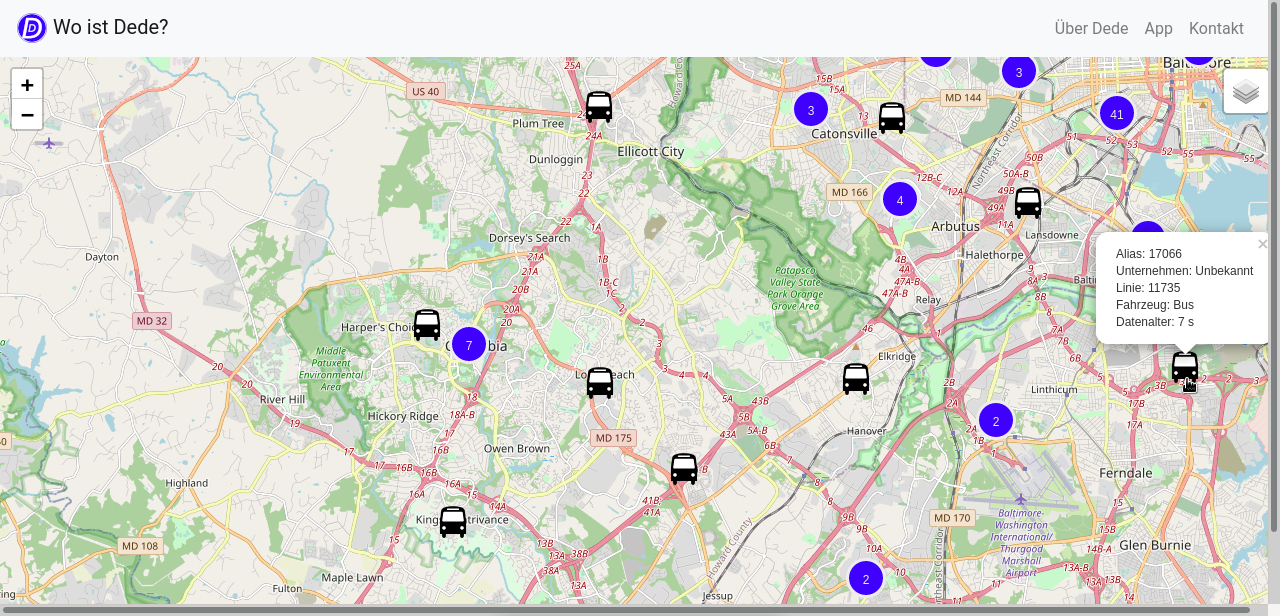
\includegraphics[width=\paperwidth]{dede/dede_real-time_map_crop}};
}

\begin{frame}{Dede Philosophie}
  Dede: eine freie, unabhängige und universelle Echtzeit-Karte
  \begin{itemize}
  \item FREI: Gemeinschaftsprojejt als freie Software (wie in Redefreiheit und NICHT wie in Freibier;-)) veröffenlicht\footnote{\url{https://github.com/dancesWithCycles/dede-front-end}}
  \item UNABHÄNGIG: weder ausgerüstete Fahrzeugflotte noch eigene IT-Infrastuktur notwendig
  \item UNIVERSELL: beliebige Fahrzeuge wie Bahn, Bus, Car-Sharing, Fahrdienst, Straßenbahn, Tram, Taxi, usw. universell darstellt
  \end{itemize}
\end{frame}

\egroup
